\clearpage
\chapter{Metodología}

\section{Desarrollo ágil de software}
  \paragraph{El desarrollo ágil propone una alternativa al desarrollo de software tradicional. Los enfoques del desarrollo ágil son principalmente usados en el desarrollo de software para ayudar a las compañias a responder fácilmente al cambio.}

\subsection{Scrum}
  \paragraph{Scrum es un marco de gestión para el desarrollo incremental de un producto que proporciona una estructura de roles, reuniones, reglas y artefactos.}
  \paragraph{Scrum utiliza iteraciones de longitud fija denominados Sprints, que son típicamente de dos semanas o 30 días de duración. Los equipos de Scrum intentan generar un incremento de producto potencialmente entregable (debidamente probado) en cada iteración.}
  
  \begin{center}
    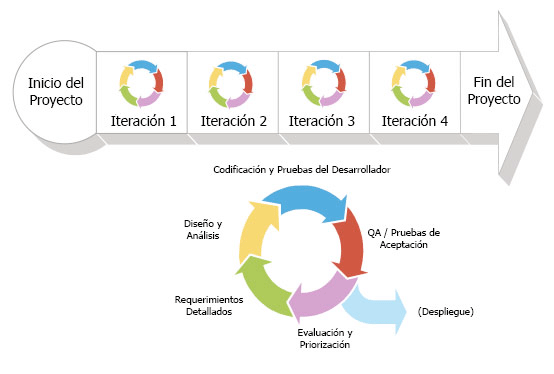
\includegraphics[width=14cm, height=9cm]{images/iterations}
  \end{center}

 \subsection{Programación Extrema (XP)}
  \paragraph{Es un enfoque disciplinado para entregar software de alta calidad rápida y continuamente. Promueve una alta participación del cliente, retroalimentación rápida, pruebas continuas, planeación continua y entrega de software funcional en intervalos muy frecuentes que van de 1 a 3 semanas.}
  
\section{Técnicas de desarrollo ágil}

\subsection{Desarrollo guiado por pruebas (Test Driven Development)}

  \paragraph{El desarrollo guiado por pruebas es una técnica avanzada qua hace uso de pruebas unitarias para guiar el diseño del software y forzar el desacoplamiento de dependencias.}
  \paragraph{El resultado de usar esta práctica es una comprensiva suite de pruebas que pueden ser ejecutadas en cualquier momento para proporcionar información de que el software está aún funcionando.}

\subsection{Refactor}
  \paragraph{Es una técnica disciplinada para la reestructuración de un cuerpo de código existente, alterando su estructura interna sin cambiar su comportamiento exterior.}
  \paragraph{Cada transformación es pequeña, pero una secuencia de transformaciones pueden producir una importante reestructuración.}

\subsection{Integración continua}
  \paragraph{Es una práctica de desarrollo que requiere a los desarrolladores la integración de código en un repositorio compartido varias veces al día.}
  \paragraph{Cada registro de entrada es entonces verificado por un proceso de construcción automatizado permitiendo a los equipos detectar problemas a tiempo.}
  \paragraph{La integración continua trae muchos beneficios, entre ellos la detección de errores rápidamente y reducir los problemas de integración lo que permite entrega de software más rápidamente.}

\section{Justificación}

Para el desarrollo del sistema pondrémos en práctica las técnicas mencionadas anteriormente que son características del marco de trabajo Scrum y de la metodología Extreme Programming.

El proceso de desarrollo del proyecto se llevará a cabo de la siguiente manera:

\begin{itemize}
  \item Planteamiento de las historias de usuario. 
  \item Definción del plazo de tiempo para cada sprint y el conjunto de funcionalidades relacionadas a cada historia de usuario que serán desarrolladas dentro del mismo.  
  \item Implementación de pruebas unitarias en conjunto con el desarrollo de cada módulo de la aplicación. 
  \item Implementación de pruebas de integración para verificar la comunicación entre dos o más modulos.
  \item Despliegue de la aplicación en un ambiente productivo una vez que todas las pruebas hayan pasado.
  \item Implementación de pruebas funcionales para verificar que el flujo descrito en las historias de usuario se lleva a cabo correctamente.
\end{itemize}
